\documentclass{article}

\usepackage[utf8]{inputenc}		% obsluga jezyka polskiego
\usepackage[MeX]{polski}		%

\usepackage[top=1in, bottom=1.25in, left=1.25in, right=1.25in]{geometry}		%zmiana marginesów

\usepackage{graphicx}		%wyswietlanie obrazow
\usepackage{float}			%

\usepackage{rotating}		%obracanie obrazow
\usepackage{tikz}			%

\usepackage{multicol}		%tekst w kolumnach

\usepackage{listings}											%obsluga wyswietlania kodu
\usepackage{xcolor}												%
\lstset { %														%
	basicstyle=\ttfamily    									%
    language=C,													%
    backgroundcolor=\color{black!5}, % set backgroundcolor		%
    basicstyle=\footnotesize,% basic font setting				%
}																%
\usepackage{minted}

\renewcommand{\labelitemi}{--}			%zmiana wygladu znacznikow wypunktowania
\renewcommand{\labelitemii}{--}		%
%\usepackage[export]{adjustbox}
\usepackage{array}


\begin{document}

\begin{titlepage} 
	\newcommand{\HRule}{\rule{\linewidth}{0.5mm}} 
	
	\center 
	
	%------------------------------------------------
	%	Headings
	%------------------------------------------------
	
	\textsc{\LARGE Wroclaw University of Science and Technology}\\[1.5cm] % Main heading such as the name of your university/college
	
	%\textsc{\Large Podstawy Techniki Mikroprocesorowej}\\[0.5cm] % Major heading such as course name
	
	%\textsc{\large Dokumentacja techniczna projektu}\\[0.5cm] % Minor heading such as course title
	
	%------------------------------------------------
	%	Title
	%------------------------------------------------
	
	\HRule\\[0.4cm]
	
	{\huge\bfseries Electronics Guidebook}\\[0.4cm] % Title of your document
	
	\HRule\\[1.5cm]
	
	%------------------------------------------------
	%	Author(s)
	%------------------------------------------------
	
	%\begin{minipage}{0.5\textwidth}
	%	\begin{flushleft}
	%		\large
	%		\textit{Autor:}\\
	%		\textsc{Maciej Mielcarski} \\numer albumu: 235703\\~\\Wydział Elektroniki W-4\\Automatyka i Robotyka 
	%	\end{flushleft}
	%\end{minipage}
	%~
	%\begin{minipage}{0.4\textwidth}
	%	\begin{flushright}
	%		\large
	%		\textit{Grupa zajęciowa:}\\
	%		\textsc{ŚR TP 13:15} 
	%	\end{flushright}
	%\end{minipage}

\vfill\vfill\vfill % Position the date 3/4 down the remaining page
	
	{\large Maciej Mielcarski \\~\\15.04.2018 issue 1.0 } % Date, change the \today to a set date if you want to be precise 
	
\end{titlepage}
\tableofcontents				% spis treści
\newpage


\pagenumbering{gobble}

  %\maketitle
  \newpage
\pagenumbering{arabic}  

\section{Introduction}
The main use of the present document is to provide compact and convenient help in form of quick descriptions, schematics, code and IC pinouts in order to simplify work with electronics. This guidebook is in constant development, any suggestions or comments can be sent to mielcarski.m@gmail.com

\section{Atmel AVR}
\subsection{ATmega models}
\begin{table}[H]
\centering
\caption{AtMega MCU comparison} 
\label{ATmega comparison}
\begin{tabular}{|l|c|c|c|c|m{1cm}|m{1cm}|m{1cm}|m{1cm}|m{1cm}|}
  \hline 
  uC name & Clock & Flash & EEPROM & SRAM & 8-bit TIM & 16-bit TIM & PWM & 10-bit ADC & GPIO \\
  \hline 
  ATmega 8 (DIP)& 16MHz & 8KB & 512B & 1KB & 2 & 1 & 3 & 6 & 23 \\
  \hline
  ATmega 32 (DIP) & 16MHz & 32KB & 1024B & 2KB & 2 & 1 & 4 & 8 & 32 \\
  \hline
  ATmega 328 (DIP) & 20MHz & 32KB & 1024B & 2KB & 2 & 1 & 4 & 6 & 23 \\
  \hline
\end{tabular} 
\end{table}

\newpage
\subsection{ATmega 8}

\begin{figure}[H]
	\center
	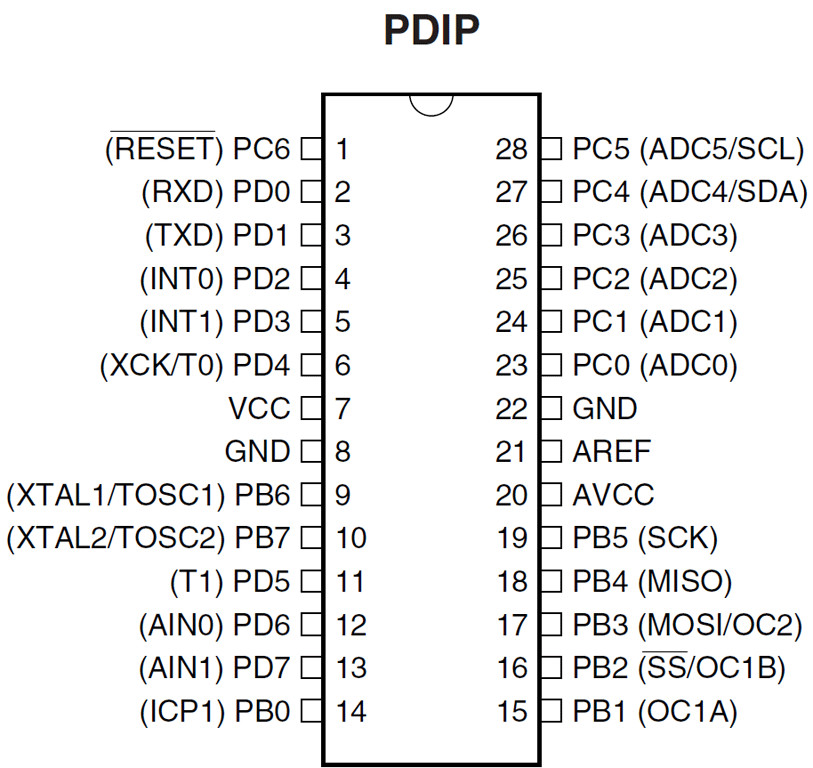
\includegraphics[scale=0.3]{img/atmega8-pinout.jpg}
	\caption{Atmega 8 wyprowadzenia}
	\label{fig:img1}
\end{figure}

\subsection{Atmega 32}
atmega 32 lorem ipsum

\begin{figure}[H]
	\center
	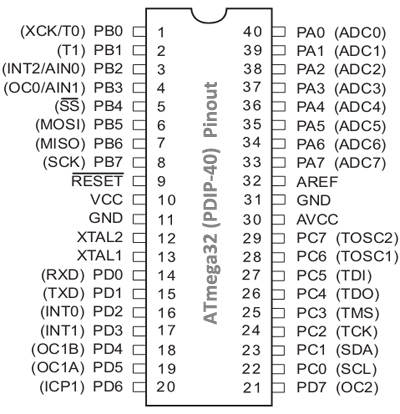
\includegraphics[scale=0.5]{img/atmega32-pinout.jpg}
	\caption{Atmega 32 wyprowadzenia}
	\label{fig:img2}
\end{figure}

\subsection{Atmega 328}
atmega 328 lorem ipsum

\begin{figure}[H]
	\center
	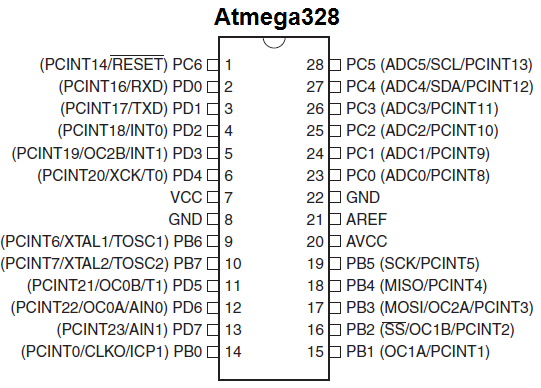
\includegraphics[scale=0.7]{img/Atmega328-pinout.png}
	\caption{Atmega 328 wyprowadzenia}
	\label{fig:img2}
\end{figure}


\subsection{Zasilanie}
zasilanie lorem ipsum

\begin{figure}[H]
	\center
	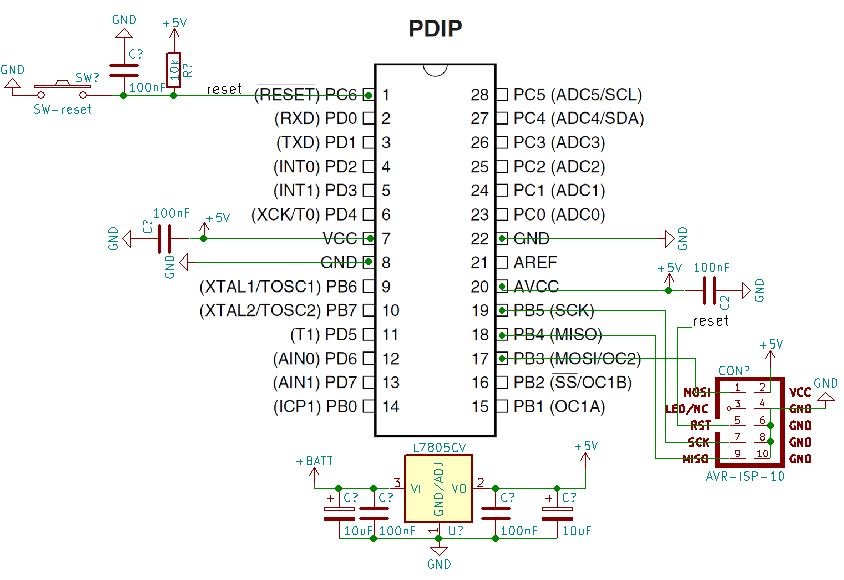
\includegraphics[width=\textwidth]{img/atmega-zasilanie.jpg}
	\caption{Atmega 8 zasilanie + programator}
	\label{fig:img3}
\end{figure}

\section{ADC}
ADC converter of a n-bit resolution is capable of converting analog signal into digital values between 0 and $2^n$ - 1.
In order to enable ADC conversion in AVR, we need to set the CPU clock prescaler and set the enable bit (according to the datasheet). For example, for atmega 328 uC, initialization of the registers is performed by this code:

\begin{minted}[tabsize=3,obeytabs]{c}
ADCSRA |= (1 << ADPS2) | (1 << ADPS1) | (1 << ADPS0); // Set ADC prescalar to 128 
ADMUX |= (1 << REFS0); 	// Set ADC reference to AVCC
ADCSRA |= (1 << ADEN);  // Enable ADC
\end{minted}
%
ADC single conversion function:
\begin{minted}[tabsize=3,obeytabs]{c}
uint16_t ADC_read(uint8_t channel)		
{
	channel &= 0x07;					// AND operation with 7 (will keep channel between 0-7) 
	ADMUX = (ADMUX & 0xF8) | channel;	// clears 3 first bits before OR

	ADCSRA |= (1 << ADSC);				// start single convesrion
	while(ADCSRA & (1 << ADSC));		// wait for conversion to complete
	return ADCW;
}
\end{minted}

\subsection{Filtering Noise}
Even though filtering all of the noise from ADC reading is impossible, there are certain measures to minimize this unwanted effect.
\subsubsection{Proper power supply connection}
In most cases, voltage reference is preferably set to internal Vcc, which requires a \textbf{LC low-pass filter} on AVcc power supply pin and \textbf{100nF capacitor to GND on Vref} pin:
\begin{figure}[H]
	\center
	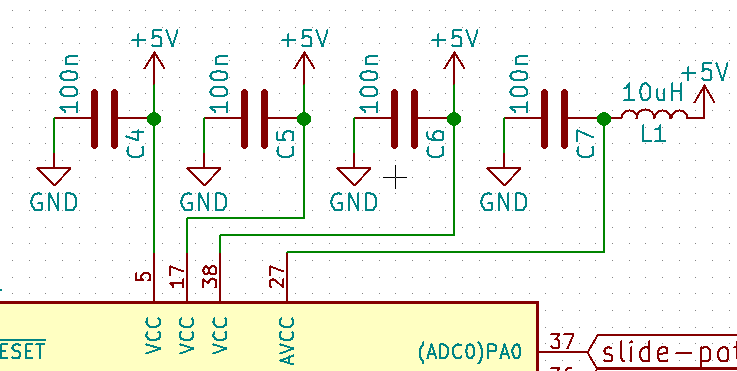
\includegraphics[scale=0.3]{img/atmega-avcc.png}
	\caption{Atmega 32 AVcc LC filter}
\end{figure}
\begin{figure}[H]
	\center
	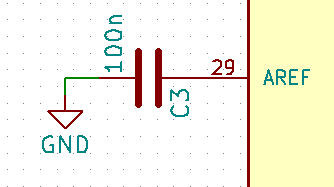
\includegraphics[scale=0.4]{img/atmega-vref.png}
	\caption{Atmega 32 Aref filtering}
\end{figure}

\subsubsection{Lowering ADC resolution}
If steadiness of ADC reading is more important for us than high resolution (eg. MIDI Control Change messages), lowering it will result in huge boost in suppresing oscillations in readings. It is simply done by \textbf{binary shifting} read ADC value. In order to \textbf{decrease} ADC resolution from \textbf{10 bit} to \textbf{7 bit}:
%
\begin{minted}[tabsize=3,obeytabs]{c}
int adc_10bit_reading = ADC_read(channel);
int adc_7bit_reading = (adc_10bit_reading>>3);
\end{minted}

\subsubsection{Averaging readings}
A batch of averaged readings may be more useful than single one. It is prefered for the number of averaged readings to be chosen as a power of 2 in order to minimize uC's computing power. Averaging \textbf{16} readings:
\begin{minted}[tabsize=3,obeytabs]{c}
int adc_sum = 0;
	for(int i=0;i<16;i++)
	{
		adc_sum += ADC_read(channel);
	}
int adc_reading = adc_sum/16;
\end{minted}

\subsubsection{Exponential moving average (EMA)}	%TODO: insert EMA formula
If our ADC reading is resisting all of the conventional methods, it may be neccesery to implement additional averaging algorithm. 
\begin{minted}[tabsize=3,obeytabs]{c}
const float EMA_a = 0.6;
int EMA = 0;
int adc_reading = 0, adc_prev_reading = 0;

adc_prev_reading = adc_reading;
adc_reading = ADC_read(channel);

EMA = (EMA_a*adc_reading) + (1-EMA_a)*adc_prev_reading;
\end{minted}

\section{USART}
Before initializing USART communication, it is required to define \textbf{CPU frequency} and desired \textbf{baud rate}, which is needed to calculate \textbf{UBRR} value, which initialises USART communication peripherals to match said frequency and baud rate: 
\begin{center}
\textit{MYUBRR = FOSC/16/BAUD-1}
\end{center}
%
USART registers initialization (atmega 328):
\begin{minted}[tabsize=3,obeytabs]{c}
UBRR0H = (unsigned char)(ubrr>>8);	// set baud rate to 9600
UBRR0L = (unsigned char)ubrr;		//
UCSR0B = (1<<RXEN0)|(1<<TXEN0);		// Enable receiver and transmitter 
UCSR0C = (1<<USBS0)|(3<<UCSZ00);		// Set frame format: 8data, 2stop bit
\end{minted}
%
Basic USART data manipulation:
\begin{minted}[tabsize=3,obeytabs]{c}
void uart_putchar(char c) 
{
	while ( !(UCSR0A & (1<<UDRE0)) )	// Wait for empty transmit buffer 
	;
    UDR0 = c;							// Put data into buffer, sends the data 
}

char uart_getchar(void) {
    loop_until_bit_is_set(UCSR0A, RXC0); 	// Wait until data exists
    return UDR0;
}

void uart_putstring(char tab[])
{
	int i =0;
	while (( UCSR0A & (1<<UDRE0))  == 0){};
        while (tab[i] != 0x00)
		{ 
            uart_putchar(tab[i]);
			i++; 
        }
}

void uart_putint(int value)
{
	char tab[16];
	itoa(value,tab,10);
	uart_putstring(tab);
}
\end{minted}
%
In oreder to communicate with computer using USART, proper \textbf{USB-RS232 Adapter} is needed. 

\section{Git}
\subsection{Creating local and remote repository}
\textbf{git init} - initialize local repository in curren directory\\
\textbf{git remote add origin $<$link.git$>$} - add remote repository\\
\textbf{git config - -global user.email $<$email adress$>$} - define user email\\
\textbf{git config - -global user.name $<$name$>$} - define user name\\

\subsection{Repository status}
\textbf{git status} - list tracked/untracked files\\
\textbf{git branch} - list all branches\\
\textbf{git log - -diff-filter=D --summary} - list all deleted files\\
\textbf{git remote -v} - list all defined remote repositories\\

\subsection{Recovery}
\textbf{git checkout $<$commit$>$$\land$ - - $<$file$>$} - recovering deleted files\\

\subsection{Commit and push}
\textbf{git add . } - add all of the untracked files\\
\textbf{git commit -m "commit description"} - commit all changes with label\\
\textbf{git push -u origin master} - push current master branch to origin remote repository\\
\section{Makefile}

\subsection{Szablony programów}
\subsubsection{Kod bazowy}

\begin{minted}[tabsize=3,obeytabs]{c}
#define F_CPU 1000000UL
#include <stdio.h>
#include <avr/io.h>
#include <util/delay.h>

int main()
{
	while(1)
	{
	
	}
	
	cout<<"hello world"<<endl;
	return 0;
}
\end{minted}

\subsubsection{Obsługa przycisku monostabilnego}

\begin{minted}[tabsize=3,obeytabs]{c}
int isButton()				//checks if encoder button is pressed
{
	if(!(PINA & 0x08))
		return 1;
	else
		return 0;
}
\end{minted}

\subsubsection{migająca dioda}

\begin{minted}[tabsize=3,obeytabs]{c}
void blinkLed(int on, int off)	// turn on the led for 
{								//'on' and off for 'off' milisecondds
	PORTC |= (1<<LED);
	delay_ms(on);
	PORTC &= ~(1<<LED);
	delay_ms(off);
}
\end{minted}

\subsubsection{Obsługa enkodera obrotowego}

\begin{minted}[tabsize=3,obeytabs]{c}

DDRA &=~ (1 << ENC_A);		// encoder pins as input
DDRA &=~ (1 << ENC_B);		//
PORTA |= (1 << ENC_B)		// with pull-up enabled
		|(1 << ENC_A);		//

uint8_t readEncoder(void)	//reads the gray code from encoder
{
 uint8_t val=0;

  if(!bit_is_clear(PINA, ENC_B))
	val |= (1<<1);

  if(!bit_is_clear(PINA, ENC_A))
	val |= (1<<0);

  return val;
}

void readEncoderCounter ()		//monitoring encoder counter 
{								//increase or decrease 
	uint8_t val_tmp = 0;						
	val_tmp = readEncoder();			

	if(val != val_tmp)
	{
		if((val==3 && val_tmp==1))
			{
			encoderCount ++;	//clockwise turn
			}
		else if((val==2 && val_tmp==0))
			{
			encoderCount --;	//counter-clockwise turn
			}
		val = val_tmp;
		}
	delay_ms(1);
}

\end{minted}

\section{Podłączenie elementów wykonawczych}
\subsection{Eliminacja drgań styków - przycisk monostabilny}

\begin{figure}[H]
	\center
	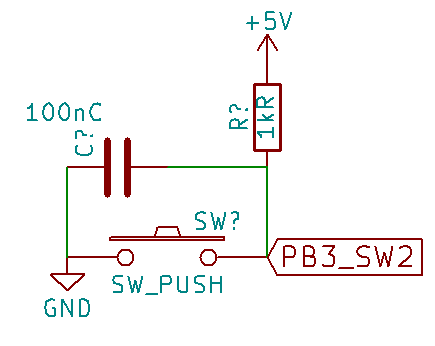
\includegraphics[scale=0.8]{img/przycisk-mono.jpg}
	\caption{kompensacja drgań styków przycisku monostabilnego}
	\label{fig:img5}
\end{figure}

\section{Arduino}
arduino lorem ipsum

\subsection{Arduino UNO}

\begin{figure}[H]
	\center
	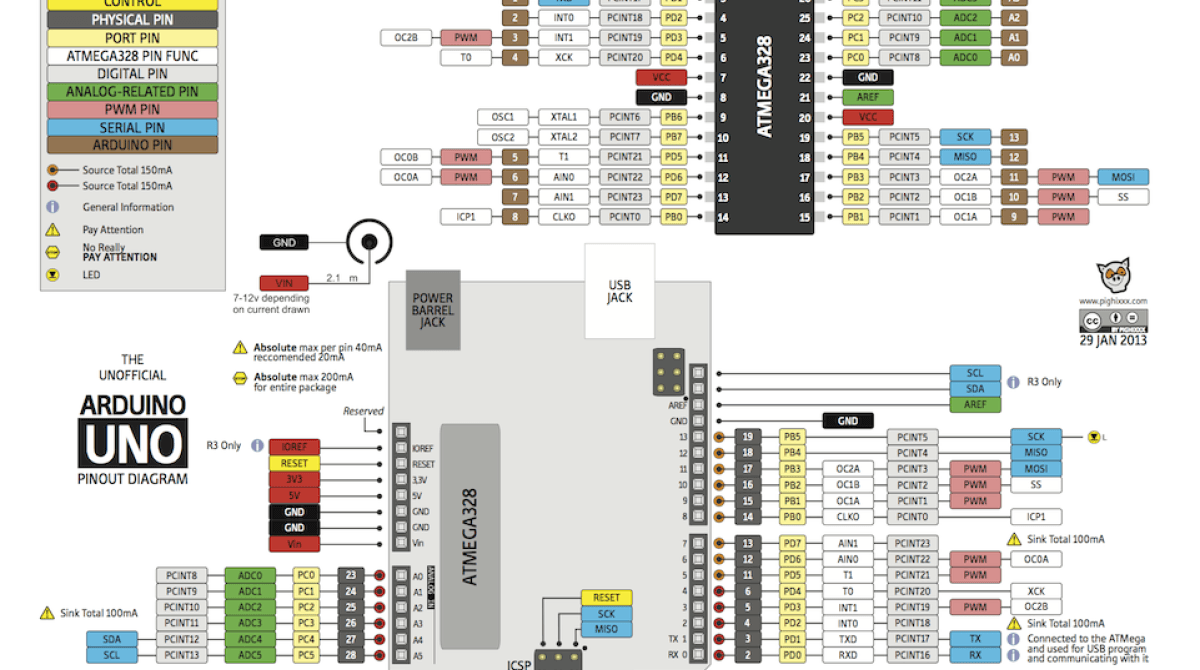
\includegraphics[scale=0.4]{img/arduino-pinout.png}
	\caption{arduino uno i atmega 328 - wyprowadzenia}
	\label{fig:img6}
\end{figure}

\begin{itemize}
	\item Arduino UNO:
\item mikrokontroler: 		ATmega328P
\item napięcie pracy: 			5V
\item napięcie zasilania: 		6-20V
\item wyjścia/wejścia cyfrowe: 	14 (w tym 6 PWM)
\item wejścia analogowe: 		6
\item wydajność prądowa pinu: 	20mA
\item pamięć Flash: 			32 KB 
\item pamięć SRAM: 			2KB
\item pamięć EEPROM: 		1KB
\item zegar: 				16 MHz
\item wymiary: 			68.6 x 53.4 mm, 25 g
\end{itemize}

\subsection{Obsługa bibliotek}
\subsubsection{Podstawowe operacje na pinach}

Biblioteka implementacji funkcji C++ : <Wire.h>\\
Obsługa pinów cyfrowych na przykładzie pinu nr 5:\\~\\

pinmode: 			pinMode(x, OUTPUT)\\
pullup				pinMode(x, INPUT\_PULLUP)\\
ustawianie stanu: 		digitalWrite(x,HIGH)\\
czytanie stanu: 			digitalRead(button)\\
opóźnienie: 			delay(50)\\

\section{MIDI}
\subsection{Podłączenie}
\begin{figure}[H]
	\center
	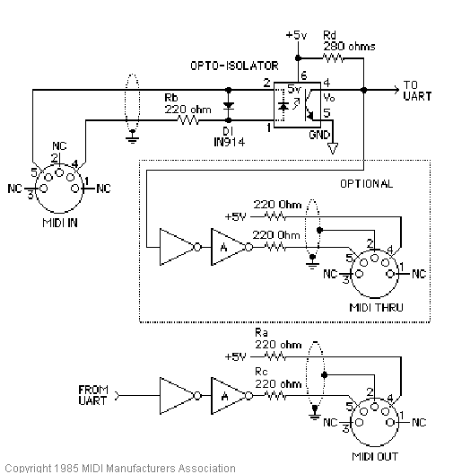
\includegraphics[scale=0.9]{img/MIDI_connection.png}
	\caption{Prawidłowe podłączenie wejścia, przejścia i wyjścia MIDI według MIDI.org}
	\label{fig:img6}
\end{figure}

\section{Konektory}
\subsection{USB}
\begin{figure}[H]
	\center
	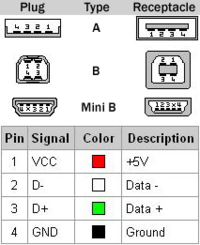
\includegraphics[scale=0.9]{img/usb-pinout.png}
	\caption{USB wyprowadzenia}
	\label{fig:img7}
\end{figure}

\subsection{AVR-ISP}
\begin{figure}[H]
	\center
	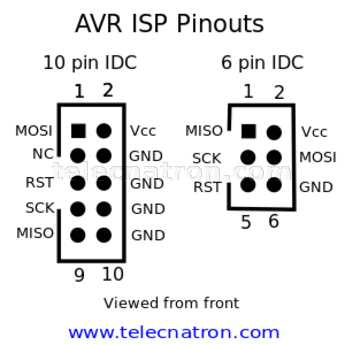
\includegraphics[scale=0.9]{img/avr-isp-pinout.png}
	\caption{AVR-ISP wyprowadzenia}
	\label{fig:img8}
\end{figure}


\end{document}
